\documentclass[9pt]{article}
\usepackage{amsmath,amsfonts,amssymb,times}
\usepackage{graphicx,color,tikz,pgfplots}
\usepackage[paperwidth=8cm,paperheight=7.2cm,lmargin=0in,rmargin=0in,tmargin=1em,bmargin=0.in]{geometry}
\usepackage{bm}
\usetikzlibrary{arrows,shadings,shapes.arrows,decorations.pathreplacing,calc}
\usepgfplotslibrary{fillbetween}


\pagestyle{empty}
\pgfplotsset{compat=newest}
\definecolor{applered}{RGB}{255,8,0}
\definecolor{azure}{RGB}{0,127,255}
\definecolor{violet}{RGB}{159,0,255}

\pgfdeclareverticalshading{rainbow}{100bp}
{color(0bp)=(applered); color(25bp)=(red); color(40bp)=(yellow);
  color(47bp)=(green); color(51bp)=(cyan); color(60bp)=(blue);
  color(65bp)=(violet); color(100bp)=(violet)} 
                          
\newlength{\h}
\newlength{\rad}
\newlength{\shorten}
\setlength{\h}{3cm}
\setlength{\rad}{4pt}
\setlength{\shorten}{2pt}

\begin{document}
\centering
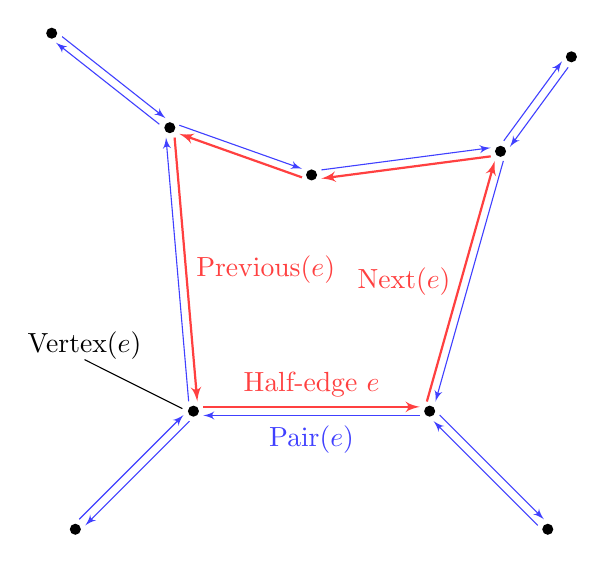
\begin{tikzpicture}[
    vertex/.style={circle, minimum width=\rad, inner sep=0pt, fill=black},
    insideEdge/.style ={thick, red!75!white,  -latex', shorten <=\shorten, shorten >= \shorten},
    outsideEdge/.style={thin, blue!75!white, -latex', shorten <=\shorten, shorten >= \shorten},
  ]

  \node[vertex, alias=v1] at (0,0) {};
  \node[vertex, alias=v2] at (\h, 0) {};
  \node[vertex, alias=v3] at (1.3\h,1.1\h) {};
  \node[vertex, alias=v4] at (0.5\h,1.\h) {};
  \node[vertex, alias=v5] at (-0.1\h,1.2\h) {};

  \draw[insideEdge] (v1.north east) -- (v2.north west) node [midway, above] {Half-edge $e$};
  \draw[insideEdge] (v2.north west) -- (v3.south west) node [midway,left, anchor=east] {$\textrm{Next}(e)$};
  \draw[insideEdge] (v3.south west) -- (v4.south east);
  \draw[insideEdge] (v4.south west) -- (v5.south east);
  \draw[insideEdge] (v5.south east) -- (v1.north east) node [midway,right, anchor=west] {$\textrm{Previous}(e)$};

  \draw[outsideEdge](v2.south west) -- (v1.south east) node [midway,below, anchor=north] {$\textrm{Pair}(e)$};
  \draw[outsideEdge](v1.north west) -- (v5.south west);
  \draw[outsideEdge](v5.north east) -- (v4.north west);
  \draw[outsideEdge](v4.north east) -- (v3.north west);
  \draw[outsideEdge](v3.south east) -- (v2.north east);

  \node[vertex, alias=u1] at (-0.5\h, -0.5\h) {};
  \node[vertex, alias=u2] at ( 1.5\h, -0.5\h) {};
  \node[vertex, alias=u3] at ( 1.6\h,  1.5\h) {};
  \node[vertex, alias=u5] at (-0.6\h,  1.6\h) {};

  \draw[outsideEdge] (u1.north) -- (v1.west);
  \draw[outsideEdge] (v1.south) -- (u1.east);

  \draw[outsideEdge] (u2.west) -- (v2.south);
  \draw[outsideEdge] (v2.east) -- (u2.north);

  \draw[outsideEdge] (u3.south) -- (v3.east);
  \draw[outsideEdge] (v3.north) -- (u3.west);

  \draw[outsideEdge] (u5.east) -- (v5.north);
  \draw[outsideEdge] (v5.west) -- (u5.south);

  \node[anchor=south east, alias=vert,inner sep=0pt,xshift=-0.2\h,yshift=0.2\h] at (v1.north west) {$\textrm{Vertex}(e)$};
  \draw[shorten >= 2pt] (vert.south) -- (v1.west);
  
\end{tikzpicture}
\end{document}
